% ---------------------------------------------------------------------------------------------------------
% 提案：双対場学習（Dual Field Learning）
% ---------------------------------------------------------------------------------------------------------
\section{提案：双対場学習}
\label{sec:dfl}
\subsection{動機：主変数ではなく双対変数を学ぶ}
世界モデル~\cite{ha2018,hafner2020}は，状態 $s$ と行動 $a$ から次の状態 $s'=f(s,a)$ を予測する関数を学習し，方策はその上で探索する．
しかし本課題のように成否が硬い物理制約（把持容量，摩擦錐，可動域，壁）で決まる運動では，
学習に必要なのは「次に何が起こるか」よりも「ここから先，どの物理制約がどれだけ効いてくるか」である．
軌道最適化の最適性条件はまさにこの情報を与える．
ある状態 $\bm x_0$ と時刻 $t_0$ から先の最適値を $J^*(\bm x_0,t_0;\bm b)$ と書く（$\bm b$ は体重，身長，筋力，装置周期などのパラメータ）．
随伴状態（costate）
\begin{equation}
\bm p^*=\frac{\partial J^*}{\partial\bm x_0}
\end{equation}
は「状態を少し変えたとき，到達できる最良の結果がどれだけ変わるか」を表し，
制約 $g_k\le0$ のラグランジュ乗数 $\lambda_k$ は「その制約を少し緩めたとき結果がどれだけ良くなるか」（影の価格）を表す．
さらに包絡線定理により，パラメータについての勾配も乗数から得られる：
\begin{equation}
\frac{\partial J^*}{\partial\bm b}=\frac{\partial\ell}{\partial\bm b}+\sum_k\lambda_k\frac{\partial g_k}{\partial\bm b}.
\label{eq:envelope}
\end{equation}
ここで $\ell$ は目的関数である．
本稿は，価値 $V=J^*$，costate $\bm p^*$，価格 $\lambda_k$ からなる\textbf{双対場}を学習の対象にすることを提案する（図~\ref{fig:dfl}）．
\begin{figure*}[t]
\centering
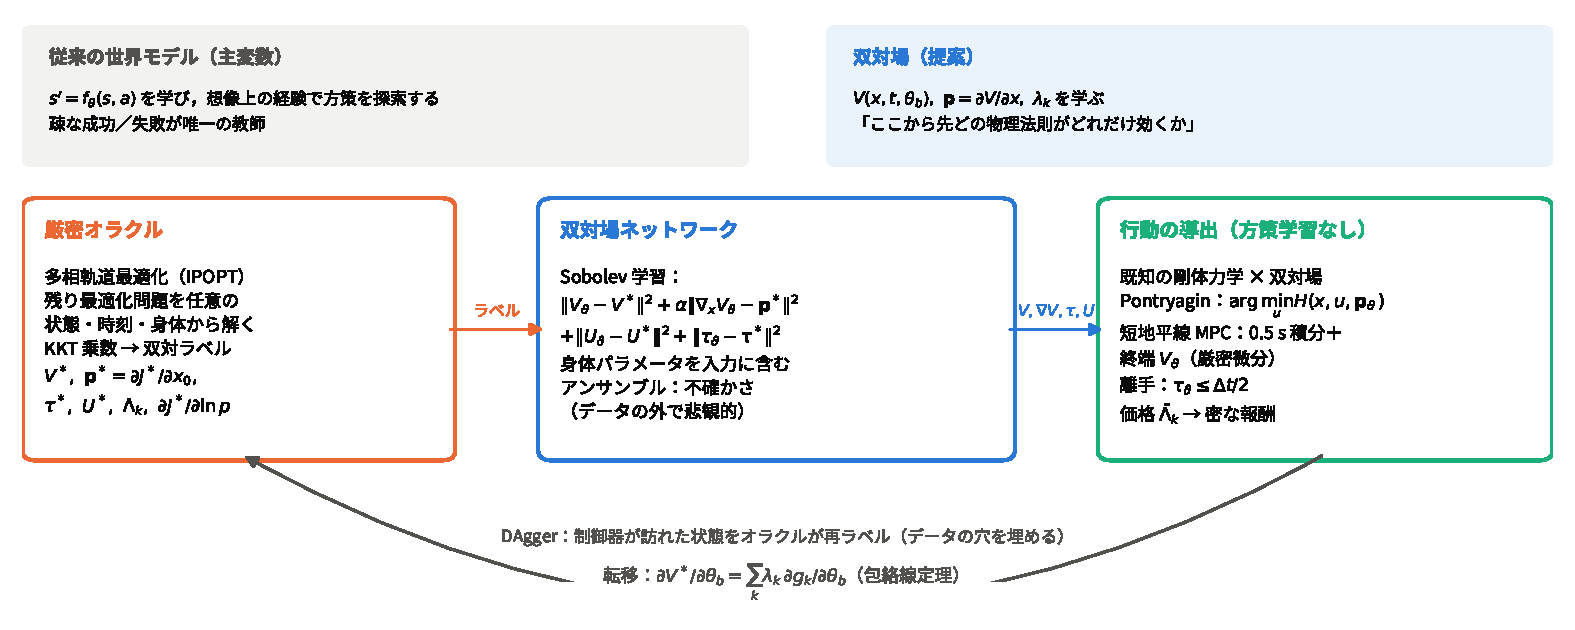
\includegraphics[width=\linewidth]{../results/figs/dfl_schematic.pdf}
\caption{双対場学習の全体像．上：状態遷移（主変数）を学ぶ従来の世界モデルと，価値・costate・価格（双対変数）を学ぶ提案の対比．
下：軌道最適化（オラクル）の乗数が双対ラベルを与え，値と勾配を同時に合わせる Sobolev 学習で場を学び，既知の力学と組み合わせて行動を決める．
制御器が実際に訪れた状態はオラクルが解き直してラベルを付ける．}
\label{fig:dfl}
\end{figure*}
状態遷移や方策を学ぶ場合と比べ，双対場は
(i)~成功か失敗かの 1 ビットではなく全状態で値と勾配をもつ密な教師であり，
(ii)~既知の力学と組み合わせれば行動に変換でき，
(iii)~式~\eqref{eq:envelope} によって体格や筋力の違う個体への一次の転移則を含む，
という性質をもつ．
本稿の検証の中心は，このうち (i) と (ii) が閉ループの成功率を実際に上げるかどうかである．

\subsection{オラクルによる双対ラベル}
第~\ref{sec:opt}節の多相軌道最適化を，任意の振りの状態 $\bm x_0=(\theta_1,\dots,\theta_5,\dot\theta_1,\dots,\dot\theta_5)$ と時刻 $t_0$ から解く
\textbf{残り最適化問題}に拡張した（待機相はなく，離手時刻は自由）．以下，この最適化器をオラクルと呼ぶ．
初期条件 $\bm X(t_0)=\bm x_0$ を等式制約として課すと，その乗数が costate $\bm p^*=\partial J^*/\partial\bm x_0$ である．
1 回の求解は，価値 $V=J^*$，その状態から先に必要な把持容量 $U^*$，最適な離手までの残り時間 $\tgo$，costate $\bm p^*$ を与える．
さらに，力学の等式制約（区間ごとの欠陥制約）の乗数は軌道上の各節点での costate に対応するので，
1 本の解から振りの全節点にラベルが得られる．
参照解の軌道上の状態（15 節点おき）と，可動域と壁の内側で摂動した状態
（角度の標準偏差 $0.06k$\,rad，角速度 $0.4k$\,rad/s，$k\in\{1,2\}$）から残り最適化問題を解いた．
求解は \dsNsolve 回（うち収束 \dsNok 回）で，\dsNref 本の参照解（$T\in\{16,\dots,19\}$\,s，$m\in\{60,\dots,75\}$\,kg）にまたがる．
ここから学習用 \fitNtrainS，検証用 \fitNvalS，未知体格用 \fitNholdS の状態ラベルを得た．

\subsection{Sobolev 学習}
双対場ネットワークは，状態 $\bm x$，装置位相 $\phi$，パラメータ $\bm b$ を入力とし，価値 $V_\vartheta$，必要容量 $U_\vartheta$，残り時間 $t_{\mathrm{go},\vartheta}$ を出力する
（活性化関数 SiLU，幅 384 の全結合 3 層）．値と勾配の両方を合わせる Sobolev 損失~\cite{czarnecki2017}
\begin{align}
\mathcal L={}&\bigl\|V_\vartheta-V\bigr\|^2+\bigl\|U_\vartheta-U^*\bigr\|^2+\bigl\|t_{\mathrm{go},\vartheta}-\tgo\bigr\|^2\nonumber\\
&+\alpha\bigl\|\nabla_{\bm x}V_\vartheta-\bm p^*\bigr\|^2
\label{eq:sobolev}
\end{align}
で学習する．各項は学習データのばらつきで正規化した．
$\alpha=1$ が提案（以下 Sobolev），$\alpha=0$ が costate ラベルを使わない対照（以下「値のみ」）である．
両者はネットワークの構造，学習データ，学習の手順がすべて同じで，違いは costate ラベルを使うかどうかだけである．
それぞれ 4 個のネットワークのアンサンブルとして学習し，乱数の種を変えて 3 回繰り返した．

\subsection{双対場からの制御：短地平 MPC}
\label{sec:mpc}
力学は既知なので，方策ネットワークは学習しない．
最も直接的な方法は，各時刻でハミルトニアン
\begin{equation}
\mathcal H(\bm u)=\frac{w_E}{t_{\mathrm{ref}}}\Bigl(\tfrac14\|\bm u\|^2+U(\bm u)^2\Bigr)+\bm p^\top\dot{\bm x}(\bm u)
\end{equation}
を指令 $\bm u$ について最小化する Pontryagin 型の制御である．
しかし 1 制御周期でトルクが価値に与える影響は小さく，$\mathcal H$ は $\bm u$ についてほぼ平坦になる．
オラクル自身の costate を使っても，復元したトルクの誤差は中央値 0.07，最大 0.6（上限を 1 とする正規化）に達した．
そこで，既知の剛体力学を地平 $T_h$ だけ先まで陽に予測し，その終端で価値を評価する短地平のモデル予測制御（MPC）を用いる：
\begin{equation}
\min_{\bm u(\cdot)}\ \int_{t}^{t+T_h}\frac{w_E}{t_{\mathrm{ref}}}\Bigl(\tfrac14\|\bm u\|^2+U^2\Bigr)dt'+\bar V_\vartheta\bigl(\bm x(t+T_h)\bigr).
\label{eq:mpc}
\end{equation}
制約はトルク上限，変化率，摩擦・引っ掛かり錐，可動域，壁，把持容量である．
終端の $\bar V_\vartheta$ はアンサンブルの平均に標準偏差の 2 倍を足した悲観的な価値で，
学習データの分布から外れた状態には追加の罰則を課す（学習データの特徴量に当てはめた 24 成分の混合ガウス分布の負の対数尤度が，
学習データの 95\,\%点を超えた分の 2 乗）．
この罰則がないと，MPC はデータの外で価値が低く外挿された状態を見つけてそこへ向かう．
終端には，残り時間の予測が地平のぶんだけ進むこと，すなわち $t_{\mathrm{go},\vartheta}(\bm x(t+T_h))=t_{\mathrm{go},\vartheta}(\bm x(t))-T_h$ を促す 2 乗の項（重み 20）も加えた．
計画の周期は 20\,ms，地平は $T_h=0.3$\,s（15 区間）で，計画は 2\,ms の制御周期に補間して実行し，計画の状態軌道を弱い PD で追従する．
離手は残り時間の予測 $t_{\mathrm{go},\vartheta}$ が制御周期の半分を下回ったときに行う．
Sobolev の場を終端に使う制御器を\textbf{双対場 MPC}，値のみの場を使う制御器を\textbf{価値 MPC} と呼ぶ．
両者で異なるのは終端の価値だけで，残り時間と必要容量の予測器，制約，求解の設定は共通にした．
